
%(BEGIN_QUESTION)
% Copyright 2015, Tony R. Kuphaldt, released under the Creative Commons Attribution License (v 1.0)
% This means you may do almost anything with this work of mine, so long as you give me proper credit

An electrical engineer calculates that the following CT will not be able to adequately drive the protective relay under fault conditions:

\begin{itemize}
\item{} CT class = {\tt C600}
\item{} CT ratio = {\tt 1200:5}
\item{} CT secondary winding resistance = {\tt 0.25 ohms}
\item{} CT secondary wire size = {\tt 10 AWG}
\item{} CT secondary wire loop length (total) = {\tt 480 feet}
\item{} Protective relay burden = {\tt 2.5 + j0 ohms}
\item{} Maximum symmetrical fault current = {\tt 15000 amps AC}
\item{} System reactance/resistance ratio = {\tt 4}
\end{itemize}

First, verify that the engineer has correctly assessed the inadequacy of this CT circuit.  Do you concur that there is a problem here, or do you think the engineer erred and this system will work fine after all?

\vskip 10pt

Suppose the engineer proposes a solution to this problem consisting of connecting {\it two} CTs in series for each line of the system, the two CTs both sensing the same line current with their secondary windings connected in series-aiding fashion like such:

$$\includegraphics[width=15.5cm]{i03097x01.eps}$$

Will this solution work or not?  Explain your reasoning.

\vskip 20pt \vbox{\hrule \hbox{\strut \vrule{} {\bf Suggestions for Socratic discussion} \vrule} \hrule}

\begin{itemize}
\item{} Does the polarity of the two series-connected CTs matter?  What would happen if you connected the two windings so their polarity marks opposed one another?
\item{} Will connecting two CTs in series affect how the protective relay must be set?  Why or why not?
\item{} Would connecting two CTs in {\it parallel} achieve the same result?  Why or why not?
\end{itemize}

\underbar{file i03097}
%(END_QUESTION)





%(BEGIN_ANSWER)

The engineer is correct on both counts: the CT circuit as designed will not adequately source the relay's burden successfully under maximum fault conditions, and the series-connected CT solution will work.
 
%(END_ANSWER)





%(BEGIN_NOTES)

\noindent
{\bf Original system:}

\begin{itemize}
\item{} Maximum internal voltage of CT secondary = {\bf 125 volts} (given X/R ratio of 4)
\item{} Secondary current under fault conditions = {\bf 62.5 A}
\item{} Maximum CT terminal voltage under fault conditions = {\bf 109.375 volts}
\item{} Relay terminal voltage required under fault conditions = {\bf 156.25 volts}
\end{itemize}

We see the CT is inadequate because its maximum terminal voltage under load is less than the voltage required at the relay terminals to drive the burden there.  Even with no wire resistance whatsoever between the CT and the relay, it still won't meet the needs of the relay.

\vskip 10pt

Connecting pairs of identical CTs in series has the effect of doubling the effective class rating (from C600 to C1200) as well as doubling the secondary winding resistance (from 0.25 ohms to 0.5 ohms).  The results are much better:

\vskip 10pt

\noindent
{\bf Dual-CT system:}

\begin{itemize}
\item{} Maximum internal voltage of CT secondary = {\bf 250 volts} (given X/R ratio of 4)
\item{} Secondary current under fault conditions = {\bf 62.5 A}
\item{} Maximum CT terminal voltage under fault conditions = {\bf 218.75 volts}
\item{} Relay terminal voltage required under fault conditions = {\bf 156.25 volts}
\end{itemize}

Here we see how the maximum CT terminal voltage easily exceeds the relay's required voltage under fault conditions.  That difference in voltage (218.75 V $-$ 156.25 V = 62.5 V) divided by the secondary fault current (62.5 A) yields a maximum value of 1.0 ohm for wire resistance.  480 feet (total) of 10 AWG copper wire only has 0.48 ohms of resistance, and so we are safe.  In fact, the total wire length could be 1000 feet and still allow proper operation because 10 AWG copper wire is about 1 ohm per thousand feet.

%INDEX% Electronics review: current transformer (CT)
%INDEX% Protective relay: CT circuit wire resistance

%(END_NOTES)


